% -----------------------------------------------------------------------------
%
% Copyright (c) 2017 Sam Cox, Roberto Sommariva
%
% This file is part of the AtChem2 software package.
%
% This file is covered by the MIT license which can be found in the file
% LICENSE.md at the top level of the AtChem2 distribution.
%
% -----------------------------------------------------------------------------

\chapter{Model Setup} \label{ch:setup}

% -------------------------------------------------------------------- %
\section{Chemical Mechanism} \label{sec:chemical-mechanism}

The chemical mechanism is the core of an atmospheric chemistry
model. In AtChem2, the chemical mechanism file is written in
\textbf{FACSIMILE format} and has the extension \texttt{.fac}. The
format is used to describe chemical reactions in the commercial
FACSIMILE Kinetic Modelling Software. Historically, this software and
the format have been closely associated with the Master Chemical Mechanism.
The \href{https://mcm.york.ac.uk/MCM/export}{extraction tool} on the
MCM website generates \texttt{.fac} files that can be directly used in
AtChem2 (Sect.~\ref{subsec:mcm-extraction}).

Since version 1.2.3, AtChem2 also supports the \textbf{KPP format} for
chemical mechanisms. The \texttt{.kpp} mechanism file, which should
have a similar format as the KPP files generated by the MCM extraction
tool, is automatically converted to a \texttt{.fac} file
(Sect.~\ref{subsec:mechanism-file}).

\subsection{FACSIMILE format} \label{subsec:facsimile-format}

Chemical reactions are described in FACSIMILE format using the
following notation:

\begin{verbatim}
% k : A + B = C + D ;
\end{verbatim}

where \texttt{k} is the rate coefficient, \texttt{A} and \texttt{B}
are the reactants, \texttt{C} and \texttt{D} are the products. The
definition of a chemical reaction in FACSIMILE starts with the
\texttt{\%} character and ends with the \texttt{;} character. The
\texttt{:} character separates the rate coefficient from the reactants
and products.

AtChem2 accepts stoichiometric coefficients in reaction definitions
since version 1.2.3. The coefficients must be written before a species
name and can be integer or decimal values, with or without a following
space. For example, the following reaction definitions are all
equivalent:

\begin{verbatim}
% k : A + A = B + B + C ;
% k : 2A = 2B + C ;
% k : 2.0A = 2.0B + C ;
% k : 2 A = 2 B + C ;
% k : 2.0 A = 2.0 B + C ;
% k : A + A = 2B + 1.0 C ;
\end{verbatim}

\textcolor{red}{\bf Important Note}: the names of the rate
coefficients and of the chemical species (products and reactants) must
begin with a letter and not with a numerical character, although
numbers may occur at other points of the variable name. This is to
avoid confusion with the stoichiometric coefficients.\\

The rate coefficient of a chemical reaction (\texttt{k}) can be a
constant number or, more commonly, is calculated as a function of
other variables: e.g., temperature (\texttt{TEMP}), air density
(\texttt{M}), water vapour (\texttt{H2O}) and other environment
variables (Sect.~\ref{sec:environment-variables}).

Comments can be inserted in the \texttt{.fac} file to document and
annotate the chemical mechanism: in FACSIMILE format, comments are
enclosed between the \texttt{*} and \texttt{;} characters, and are
ignored by the build scripts. A basic chemical mechanism, with
comments and calculated rate coefficients, has the following format:

\begin{verbatim}
* Tropospheric O3-NOx cycle ;
* Kinetic data from Atkinson et al., ACP, 2004 ;
*;
% J_NO2                      : NO2 = NO + O ;
% 5.6D-34*M*(TEMP/300)@-2.6  : O + O2 = O3 ;
% 1.4D-12*EXP(-1310/TEMP)    : NO + O3 = NO2 + O2 ;
\end{verbatim}

In the example above, the photolysis rate of \cf{NO2}
(\texttt{J\_NO2}) can be calculated by AtChem2 as function of
latitude, longitude and solar zenith angle, or can be provided
by the user (Sect.~\ref{sec:photolysis-rates}).

Complex mathematical expressions can be used to calculate the rate
coefficients, in which case they have to be defined before the
chemical reactions that use them (typically, these are combination
or dissociation reactions). For example:

\begin{verbatim}
* Formation of nitric acid (HNO3) in the gas-phase ;
*;
* Rate coefficient (Atkinson et al., ACP, 2004) ;
K80 = 3.3D-30*M*(TEMP/300)@-3.0 ;
K8I = 4.1D-11 ;
KR8 = K80/K8I ;
FC8 = 0.4 ;
NC8 = 0.75-1.27*(LOG10(FC8)) ;
F8 = 10@(LOG10(FC8)/(1+(LOG10(KR8)/NC8)**2)) ;
KMT08 = (K80*K8I)*F8/(K80+K8I) ;
*;
* Chemical Reaction ;
% KMT08 : OH + NO2 = HNO3 ;
\end{verbatim}

Chemical reactions can also be written in FACSIMILE format without
reactants or products. This feature can be used to implement simple
descriptions of non-chemical processes in a box-model. For example,
dilution (Sect.~\ref{subsec:dilute}), surface deposition and direct
emission of a chemical species can be parametrized as:

\begin{verbatim}
* Deposition velocity of O3 = 1.4 cm s-1 ;
* Boundary layer height (BLHEIGHT) in cm ;
% 1.4/BLHEIGHT  :  O3 =  ;
*;
* Emission rate of NO2 = 1e8 molecule cm-3 s-1 ;
% 1D+8  :  = NO2  ;
\end{verbatim}

More sophisticated approaches to describe non-chemical processes can
be implemented by defining complex mathematical expressions to
calculate the corresponding ``rate coefficients'', as explained above.
Alternatively, since version 1.2.3, AtChem2 allows the user to create
custom Fortran functions: for detailed instructions, go to
Sect.~\ref{subsec:custom-functions}.

During the \hyperref[subsec:build-process]{build process}, the
chemical mechanism file has to be parsed by the \texttt{mech\_converter.py}
script, which expects the chemical mechanism file to have four sections:

\begin{description}
\item[Generic rate coefficients]: contains the equations of the
  generic rate coefficients, typically used when experimental or
  theoretical kinetic data are not available.
\item[Complex reactions]: contains the equations of the complex rate
  coefficients (e.g., for combination/dissociation reactions or
  parametrized non-chemical processes).
\item[Peroxy radicals]: contains the calculation of the sum of organic
  peroxy radicals (\cf{RO2}) -- go to Sect.~\ref{subsec:ro2-sum} for
  details.
\item[Reaction definitions]: contains the definitions of the chemical
  reactions and of the parametrized non-chemical processes (e.g.,
  aerosol uptake, dry deposition, etc\ldots).
\end{description}

For the \texttt{mech\_converter.py} script to work, the beginning of
each section must be delimited by a header constituted by a single
comment line. The header must always be present, even though the
corresponding section can be empty (e.g., if a mechanism other than
the MCM is used). Minimal chemical mechanism files
(\texttt{mechanism\_skel.*}) can be found in the \texttt{mcm/}
directory for reference. In addition, an example chemical mechanism
downloaded from the MCM website (\texttt{mechanism.fac}) is included
in the \texttt{model/} directory.

\subsection{\cf{RO2} sum} \label{subsec:ro2-sum}

The sum of organic peroxy radicals (\cf{RO2}) is a key feature of the
Master Chemical Mechanism. Organic peroxy radicals react with
\cf{HO2}, with themselves and with other organic peroxy radicals:
given that there are over 1000 \cf{RO2} in the MCM, the number of
possible self- and cross-reactions of these species is of the order of
$10^6$, which presents a significant computational challenge. The
\cf{RO2} sum is used in the MCM to reduce the number of peroxy
radicals permutation reactions. More information can be found in the
MCM protocol papers \citep{jenkin_1997, saunders_2003}.

AtChem2 is primarily designed to run box models based upon the Master
Chemical Mechanism and, therefore, the \texttt{.fac} file must contain
the \textbf{Peroxy radicals} section, as explained in
Sect.~\ref{subsec:facsimile-format}. This section must have a header
and has the following format:

\begin{verbatim}
* Peroxy radicals. ;
RO2 = RO2a + RO2b + RO2c + ... ;
\end{verbatim}

where \texttt{RO2a}, \texttt{RO2b}, \texttt{RO2c}, are the organic
peroxy radicals in the chemical mechanism. If there are no organic
peroxy radicals in the chemical mechanism (or if the mechanism is not
based upon the MCM), the \cf{RO2} sum section must still be present in
the \texttt{.fac} file, but it is left empty:

\begin{verbatim}
* Peroxy radicals. ;
RO2 = ;
\end{verbatim}

The \cf{RO2} sum is automatically generated from the \texttt{.fac}
file during the \hyperref[subsec:build-process]{build process}. The
script \texttt{mech\_converter.py} compares the list of species in the
\textbf{Peroxy radicals} section of the \texttt{.fac} file with the
list of \cf{RO2} extracted from the MCM database, which is included in
the \texttt{mcm/} directory. By default, AtChem2 uses the MCM v3.3.1;
the corresponding list of organic peroxy radicals is in the
\texttt{peroxy-radicals\_v3.3.1} file. Lists of organic peroxy
radicals for other versions of the MCM are included in the
\texttt{mcm/} directory; instructions on how to change the MCM version
can be found in the \texttt{mcm/INFO.md} file.

If one or more chemical species are included in the \textbf{Peroxy radicals}
section of the \texttt{.fac} file, but is not present in the list of \cf{RO2}
extracted from the MCM database, the \texttt{mech\_converter.py} script
prints a warning message to the terminal:

\begin{verbatim}
        !!! WARNING !!!
  The following species are not present in the RO2 reference list:
    speciesX speciesY
  Should they be included in the RO2 sum?
\end{verbatim}

In this case, the user must check manually whether the species in
question are organic peroxy radicals, amend the \textbf{Peroxy radicals}
section of the \texttt{.fac} file accordingly, and rerun the
\texttt{build\_atchem2.sh} script.

It is important to ensure that the \cf{RO2} sum is accurate, because
many reactions in the MCM depend on this parameter. This means that
all the organic peroxy radicals in the chemical mechanism must be
included in the \cf{RO2} sum, and that the \cf{RO2} sum must include
only organic peroxy radicals~\footnote{The hydroperoxyl radical
  (\cf{HO2}) is a peroxy radical but is not an organic molecule, and
  therefore it \emph{must not} be included in the \cf{RO2} sum.}. The
model calculates the \cf{RO2} sum at runtime and, by default, outputs
the value of this variable to the \texttt{environmentVariables.output}
file (Sect.~\ref{sec:output}).

\subsection{MCM extraction} \label{subsec:mcm-extraction}

The \href{https://mcm.york.ac.uk/MCM/}{MCM website} provides a
convenient tool to download the whole Master Chemical Mechanism, or
subsets of it, in FACSIMILE format. A brief overview of the process is
given here; more information can be found on the MCM website.

First, select the species of interest using the
\href{https://mcm.york.ac.uk/MCM/browse}{MCM browser} and add them to
the ``Marklist''. Then proceed to the
\href{https://mcm.york.ac.uk/MCM/export}{MCM export tool} and select
the option ``FACSIMILE'' as output format. Make sure to also select
the following options, so that all the required headers
(Sect.~\ref{subsec:facsimile-format}) are included in the generated
\texttt{.fac} file: :

\begin{verbatim}
[x] Include inorganic reactions?
[x] Include generic rate coefficients?
\end{verbatim}

Click on the ``Download'' button and save the \texttt{.fac} file into
a directory of choice -- such as the \texttt{model/} directory
(Sect.~\ref{subsec:model-directory}). The procedure to generate the
chemical mechanism file is identical if a \texttt{.kpp} file is
desired (just select the option ``KPP'' instead of ``FACSIMILE'' as
output format). The chemical mechanism file downloaded from the MCM
website is a simple ASCII text file and is ready to be used in
AtChem2. If modifications are required (e.g., chemical reactions to be
added, deleted or modified), the user can open the file with a text
editor and modify the chemical mechanism as needed.

\subsection{Custom Functions} \label{subsec:custom-functions}

The Fortran file \texttt{customRateFuncs.f90} allows the user to
define custom functions that can be called from within the chemical
mechanism to enhance the capability of the model~\footnote{\emph{N.B.}:
  this feature is available only in AtChem2 v1.3-dev and later.}. These
functions can be used to parametrize heterogeneous reactions, aerosol
formation, surface deposition, emissions and other non-chemical
processes, as discussed in Sect.~\ref{subsec:facsimile-format}.

By default, \texttt{customRateFuncs.f90} is located in
\texttt{model/configuration/} and contains an empty Fortran module
which can be modified by the user to add any number of custom
functions. During the build process, the \texttt{mech\_converter.py}
script identifies the names of all the custom functions added to the
module and includes them into the \texttt{mechanism.f90} file
(Sect.~\ref{subsec:build-process}). If no custom functions have been
defined, the content of the module is ignored.

Note that the custom functions must be defined as Fortran functions
and not as subroutines, i.e. the Fortran keyword \textbf{function}
must be used in the declaration. Environment variables
(Sect.~\ref{sec:environment-variables}), such as temperature and
pressure, can be used as arguments in a custom function. Below is an
example of a modified \texttt{customRateFuncs.f90} file which defines
a basic function to add two numbers:

\begin{verbatim}
module custom_functions_mod
  implicit none

contains

  ! Function to multiply two numbers
  pure function multiplyNumbers( inNum1, inNum2 ) result ( outNum )
    real, intent(in) :: inNum2, inNum1
    real :: outNum

    outNum = inNum1 * inNum2

    return
  end function multiplyNumbers

end module custom_functions_mod
\end{verbatim}

The ``multiplyNumbers()'' function can then be called in the
\texttt{.fac} file, together with the regular FACSIMILE notation
(Sect.~\ref{subsec:facsimile-format}). For example:

\begin{verbatim}
% multiplyNumbers(2.0, 0.5) : A = B ;
\end{verbatim}

It is the user's responsibility to ensure that the custom Fortran code
is correct. Optionally, but recommended, the Python scripts
\texttt{fix\_style.py} and \texttt{fix\_indent.py} in the \texttt{tools/}
directory can be used to check that the Fortran code follows the
AtChem2 \hyperref[subsec:style-recommendations]{coding guidelines},
which are described in Sect.~\ref{sec:style-guide}.

\subsection{Build process} \label{subsec:build-process}

AtChem2 is built using the scripts in the \texttt{build/}
directory. Here, the build process is only outlined; more detailed
instructions can be found in Sect.~\ref{sec:build}.

The Python script \texttt{mech\_converter.py} -- called by the
\texttt{build\_atchem2.sh} script -- converts the chemical mechanism
into a Fortran-compatible format. In doing so, the build script
generates a number of files:

\begin{itemize}
\item \texttt{mechanism.f90} contains the Fortran equations to
  calculate the rate coefficients of each reaction in the chemical
  mechanism.
\item \texttt{mechanism.o} is the compiled Fortran code and
  \texttt{mechanism.so} is the shared library, i.e. the pre-compiled
  chemical mechanism.
\item \texttt{mechanism.species} contains the chemical species in the
  chemical mechanism. The file has no header. The first column is the
  ID number of the species, the second column is the name of the
  species:
  \begin{verbatim}
  1 O
  2 O3
  3 NO
  4 NO2
  \end{verbatim}
\item \texttt{mechanism.reac} and \texttt{mechanism.prod} contain the
  reactants and the products (respectively) of each reaction in the
  chemical mechanism. The files have a one line header with the total
  number of species and reactions in the mechanism, and the total
  number of equations in the \textbf{Generic rate coefficients} and
  \textbf{Complex reactions} sections of the \texttt{.fac} file
  (Sect.~\ref{subsec:facsimile-format}). The first column is the ID
  number of the reaction, the second column is the ID number of the
  species (from \texttt{mechanism.species}) which is a
  reactant/product in that reaction, the third column is the
  stoichiometric coefficient of the reaction:
  \begin{verbatim}
  29 71 139 numberOfSpecies numberOfReactions numberOfGenericComplex
  1 1 1.0
  2 1 1.0
  3 1 1.0
  3 2 1.0
  \end{verbatim}
\item \texttt{mechanism.ro2} contains the organic peroxy radicals
  (\cf{RO2}) in the chemical mechanism. The file has a one line header
  as a Fortran comment. The first column is the ID number of the
  peroxy radical (from \texttt{mechanism.species}), the second column
  is the name of the peroxy radical as a Fortran comment:
  \begin{verbatim}
  ! Note that this file is automatically generated by
    build/mech_converter.py -- Any manual edits to this file
    will be overwritten when calling build/mech_converter.py
  23 !CH3O2
  26 !C2H5O2
  28 !IC3H7O2
  29 !NC3H7O2
  \end{verbatim}
\end{itemize}

The directory containing the files generated by the build script is,
by default, \texttt{model/configuration/} but its location can be changed
using the second argument of \texttt{build\_atchem2.sh}, as explained
in Sect.~\ref{sec:build} (see also Sect.~\ref{subsec:model-directory}).
The shared library (\texttt{mechanism.so}) is created in the
\sharedir, which is the same as the model configuration directory
unless otherwise specified.

% -------------------------------------------------------------------- %
\section{Model Parameters} \label{sec:model-parameters}

The model parameters control the general setup of the model, such as
the runtime, the interpolation methods, the output frequencies,
etc\ldots The model parameters, which are described below, are set in
the \texttt{model.parameters} file (by default, located in the
\texttt{model/configuration/} directory).

\begin{itemize}
\item \textbf{number of steps}, \textbf{step size}. The model runtime
  is determined by the number of steps and by the step size (in
  seconds). The step size controls the frequency of the model output
  for the chemical species listed in \texttt{outputSpecies.config}
  (Sect.~\ref{subsec:outputspecies}), as well as for the environment
  variables, the photolysis rates and the diagnostic variables. Note
  that the step size is \emph{distinct} from the integration step,
  which is independently controlled by CVODE.\\
  For example, a model run of 2 hours, with output every 5 minutes,
  requires 24 steps with a step size of 300 seconds:
  $24 \times 300 = 7200~\mathrm{seconds} = 2~\mathrm{hours}$
\item \textbf{species interpolation method}, \textbf{conditions interpolation method}.
  Interpolation method used for the constrained chemical species, and
  for the constrained environment variables and the photolysis rates,
  respectively. Two interpolation methods are currently implemented in
  AtChem2: piecewise constant and piecewise linear
  (Sect.~\ref{subsec:interpolation}). The default option is \texttt{2}
  (piecewise linear interpolation).
\item \textbf{rates output step size}. Frequency (in seconds) of the
  model output for the production and loss rates of selected species --
  listed in \texttt{outputRates.config} (Sect.~\ref{subsec:outputrates}).
  This is used for the rate of production and destruction analysis
  (ROPA/RODA, Sect.~\ref{subsec:ropa-roda}).
\item \textbf{model start time}. Start time of the model (in seconds)
  calculated from midnight of the \textbf{day}, \textbf{month},
  \textbf{year} parameters -- see below.\\
  For example, a start time of 3600 means the model run starts at 1:00
  in the morning and a start time of 46800 means the model run starts
  at 1:00 in the afternoon (13:00). The \textbf{model stop time} does
  not need to be specified: it is automatically calculated by the
  model as:
  \begin{center}
    stop time = start time + (number of steps * step size)
  \end{center}
  Note that when one or more variables are constrained, the time
  interval between the model start time and stop time \emph{must be}
  equal to, or less than, the time interval of the constrained data --
  go to Sect.~\ref{subsec:interpolation} for more information.
\item \textbf{jacobian output step size}. Frequency (in seconds) of
  the model output for the Jacobian matrix. If this parameter is set
  to \texttt{0} (default option), the Jacobian is not saved. The
  \texttt{jacobian.output} file generated by the model can be very
  large, especially if the chemical mechanism has many reactions
  and/or the model runtime is long. Therefore it is recommended to
  output the Jacobian matrix only if needed.
\item \textbf{latitude} and \textbf{longitude}. Geographical
  coordinates (in degrees). Latitude North is positive and latitude
  South is negative; longitude East is negative and longitude West is
  positive~\footnote{The standard geographical convention is that
    longitude East is positive and longitude West is negative. AtChem2
    uses the opposite convention for reasons of backward
    compatibility. This may change in future versions of
    AtChem2.}. Latitude and longitude are used to calculate the solar
  angles, which are needed for the calculation of the photolysis rates
  (Sect.~\ref{subsec:calculated-photolysis-rates}).
\item \textbf{day} and \textbf{month} and \textbf{year}. Start date of
  the model simulation. The model time is in UTC (i.e. GMT timezone)
  and is calculated in seconds since midnight of the start date.
\item \textbf{reaction rates output step size}. Frequency (in seconds)
  of the model output for the reaction rates of every reaction in the
  chemical mechanism. By default, they are saved in the
  \texttt{reactionRates/} sub-directory of \texttt{model/output}
  (Sect.~\ref{sec:output}). Note that this parameter is different from
  \textbf{rates output step size} (see above), which sets the output
  frequency for the production and loss rates of a limited number of
  species of interest.
\end{itemize}

% -------------------------------------------------------------------- %
\section{Solver Parameters} \label{sec:solver-parameters}

The solver parameters control the behaviour of the ordinary
differential equations (ODE) solver, and are set in the
\texttt{solver.parameters} file (by default, located in the
\texttt{model/configuration/} directory). A complete explanation of
these parameters can be found in the documentation of
\href{https://computing.llnl.gov/projects/sundials/cvode}{CVODE}.

\begin{itemize}
\item \textbf{atol} (positive real) and \textbf{rtol} (positive real):
  absolute and relative tolerance values for the solver.
\item \textbf{delta main} (positive real): linear convergence
  tolerance factor of the GMRES linear solver.
\item \textbf{lookback} (positive integer): maximum Krylov subspace
  dimension of the GMRES linear solver.
\item \textbf{maximum solver step size} (positive real): maximum size
  of the timesteps that the solver is allowed to use (in seconds).
\item \textbf{maximum number of steps in solver} (positive integer):
  maximum number of steps used by the solver before reaching
  \texttt{tout}, i.e. the next output time.
\item \textbf{solver type} (integer): selection of the linear solver
  to use: \texttt{1} for GMRES, \texttt{2} for GMRES preconditioned
  with a banded preconditioner (default option), \texttt{3} for a
  dense solver.
\item \textbf{banded preconditioner upper bandwidth} (integer): only
  used in the case that \texttt{solver\ type\ =\ 2}.
\item \textbf{banded preconditioner lower bandwidth} (integer): only
  used in the case that \texttt{solver\ type\ =\ 2}.
\end{itemize}

% -------------------------------------------------------------------- %
\section{Environment Variables} \label{sec:environment-variables}

The environment variables define the physical parameters of the model, such
as temperature, pressure, humidity, solar angles, boundary layer height,
etc\ldots These variables are set in the \texttt{environmentVariables.config}
file which, by default, is in the \texttt{model/configuration/} directory.

The environment variables can have a fixed value, i.e. a numerical or
logical constant, or can be constrained to a timeseries of measured
values (\texttt{CONSTRAINED}), depending on their type. If a variable
is constrained, the corresponding data file must be present in
the \texttt{model/constraints/environment/} directory
(Sect.~\ref{subsec:constrained-variables}). Some environment variables
can be calculated by the model (\texttt{CALC}) and some can be
deactivated if they are not needed (\texttt{NOTUSED}).

By default, the environment variables are either set to
\texttt{NOTUSED} or to a fixed value. The environment variables used
in AtChem2 are described below, together with their possible settings,
units, and default values.

\subsection{TEMP} \label{subsec:temp}

Ambient Temperature (K).

\begin{itemize}
\item fixed value\\$\hookrightarrow$ default: 288.15
\item constrained
\end{itemize}

\subsection{PRESS} \label{subsec:press}

Ambient Pressure (mbar).

\begin{itemize}
\item fixed value\\$\hookrightarrow$ default: 1013.25
\item constrained
\end{itemize}

\subsection{RH} \label{subsec:rh}

Relative Humidity (\%). It is required only if
\hyperref[subsec:h2o]{\texttt{H2O}} (see below) is set to
\texttt{CALC}, otherwise it must be set to \texttt{NOTUSED}.

\begin{itemize}
\item fixed value
\item constrained
\item not used\\$\hookrightarrow$ default: \texttt{NOTUSED} (-1)
\end{itemize}

\subsection{H2O} \label{subsec:h2o}

Water Concentration (molecule cm$^{-3}$). If \texttt{H2O} is set to
\texttt{CALC}, then \hyperref[subsec:rh]{\texttt{RH}} (see above) must
be set to a fixed value or \texttt{CONSTRAINED}.

\begin{itemize}
\item fixed value\\$\hookrightarrow$ default: 4.45e+17
\item constrained
\item calculated
\end{itemize}

\subsection{DEC} \label{subsec:dec}

Sun Declination (radians) is the angle between the center of the sun
and Earth's equatorial plane.

\begin{itemize}
\item fixed value
\item constrained
\item calculated\\$\hookrightarrow$ default: \texttt{CALC}
\end{itemize}

\subsection{BLHEIGHT} \label{subsec:blheight}

Boundary Layer Height. It is required only if the model includes
non-chemical processes such as the emission or deposition of chemical
species. The unit is centimetre (cm) or metre (m), depending on how
these processes are parametrized in the chemical mechanism -- go to
Sect.~\ref{subsec:facsimile-format} for details.

\begin{itemize}
\item fixed value
\item constrained
\item not used\\$\hookrightarrow$ default: \texttt{NOTUSED} (-1)
\end{itemize}

\subsection{ASA} \label{subsec:asa}

Aerosol Surface Area. It is required only if the model includes
heterogeneous chemical reactions. The unit is area (e.g., cm$^2$,
$\mu$m$^2$, nm$^2$) per volume (e.g., m$^3$, cm$^3$), depending on how
these reactions are implemented in the chemical mechanism.

\begin{itemize}
\item fixed value
\item constrained
\item not used\\$\hookrightarrow$ default: \texttt{NOTUSED} (-1)
\end{itemize}

\subsection{DILUTE} \label{subsec:dilute}

Dilution Rate (s$^{-1}$). It is required only if the model includes
the dilution of chemical species.

\begin{itemize}
\item fixed value
\item constrained
\item not used\\$\hookrightarrow$ default: \texttt{NOTUSED} (-1)
\end{itemize}

When \texttt{DILUTE} is set to a fixed value or constrained, the
chemical mechanism is automatically modified during the
\hyperref[subsec:build-process]{build process}: for each species in
the chemical mechanism, a ``loss reaction'' is added to the mechanism
with a ``rate coefficient'' equal to the dilution rate~\footnote{The
  behaviour of \texttt{DILUTE} was changed with the release of version
  1.2. Previously, the user had to manually add to the chemical
  mechanism a ``reaction'' using \texttt{DILUTE} for each species for
  which dilution was required. The new approach makes the use of
  \texttt{DILUTE} both more intuitive and more accurate.}. For
example, the following ``reactions'' are added to the ``Tropospheric
O3-NOx cycle'' mechanism shown in Sect.~\ref{subsec:facsimile-format}:

\begin{verbatim}
% DILUTE : NO2 = ;
% DILUTE : NO = ;
% DILUTE : O = ;
% DILUTE : O3 = ;
\end{verbatim}

Note that AtChem2 treats molecular oxygen (\cf{O2}) and nitrogen
(\cf{N2}) as model parameters rather than chemical species. Their
concentrations are calculated by the model as a function of
temperature and pressure and, therefore, \texttt{DILUTE} is not
applied to \cf{O2} and \cf{N2}.

\subsection{JFAC} \label{subsec:jfac}

Correction factor used to adjust the photolysis rates -- e.g., to
account for the effect of clouds. \texttt{JFAC} can have a value
between \texttt{0} (photolysis rates are set to zero) and \texttt{1}
(photolysis rates are not corrected). \texttt{JFAC} is not applied to
constant or constrained photolysis rates (Fig.~\ref{fig:photol}). For
detailed information on this parameter, go to
Sect.~\ref{subsec:jfac-calculation}.

\begin{itemize}
\item fixed value\\$\hookrightarrow$ default: 1
\item constrained
\item calculated
\end{itemize}

\subsection{ROOF} \label{subsec:roof}

Flag to switch the photolysis rates on/off. It is needed mostly for
simulations of some environmental chamber experiments, where the roof
of the chamber can be opened/closed or the lamps can be turned on/off.
When \texttt{ROOF} is set to \texttt{CLOSED} all the photolysis rates
are set to zero, including those that are constant or constrained:
this is different than setting \texttt{JFAC} to \texttt{0}, which only
applies to the calculated photolysis rates (Fig.~\ref{fig:photol}).

The parameter \texttt{ROOF} can be set only to \texttt{OPEN} (default)
or \texttt{CLOSED} and cannot be constrained.

% -------------------------------------------------------------------- %
\section{Photolysis Rates} \label{sec:photolysis-rates}

The photolysis rates are the rate coefficients of the photolysis reactions,
and are indicated in \hyperref[subsec:facsimile-format]{FACSIMILE format}
with the notation \texttt{J<i>} -- where \texttt{i} is the ID number
assigned by the MCM to each photolysis reaction (or to a group of
photolysis reactions, as per MCM protocol). AtChem2 implements the MCM
parametrization (Sect.~\ref{subsec:calculated-photolysis-rates}) to
calculate the photolysis rates; for a comparison between calculated
and measured photolysis rates, see \citet{sommariva_2020}.
Alternatively, the photolysis rates can be set to a constant value or
constrained to measured data. The following rules apply:

\begin{enumerate}
\item If a photolysis rate is set to a constant value, it assumes the
  given value; the other photolysis rates are set to zero.
\item If a photolysis rate is constrained, it assumes the values in
  the corresponding constraint file; the other photolysis rates are
  calculated.
\item If no photolysis rate is set to constant or constrained, the
  model calculates all photolysis rates.
\end{enumerate}

Fig.~\ref{fig:photol} shows how AtChem2 combines constant, constrained
and calculated photolysis rates, as well as the usage of the photolysis
correction factor \texttt{JFAC} (Sect.~\ref{subsec:jfac-calculation}).
In addition, the environment variable \texttt{ROOF} can be used to turn
the photolysis rates ON or OFF, as explained in Sect.~\ref{subsec:roof}.

\begin{figure}[htb]
  \centering
  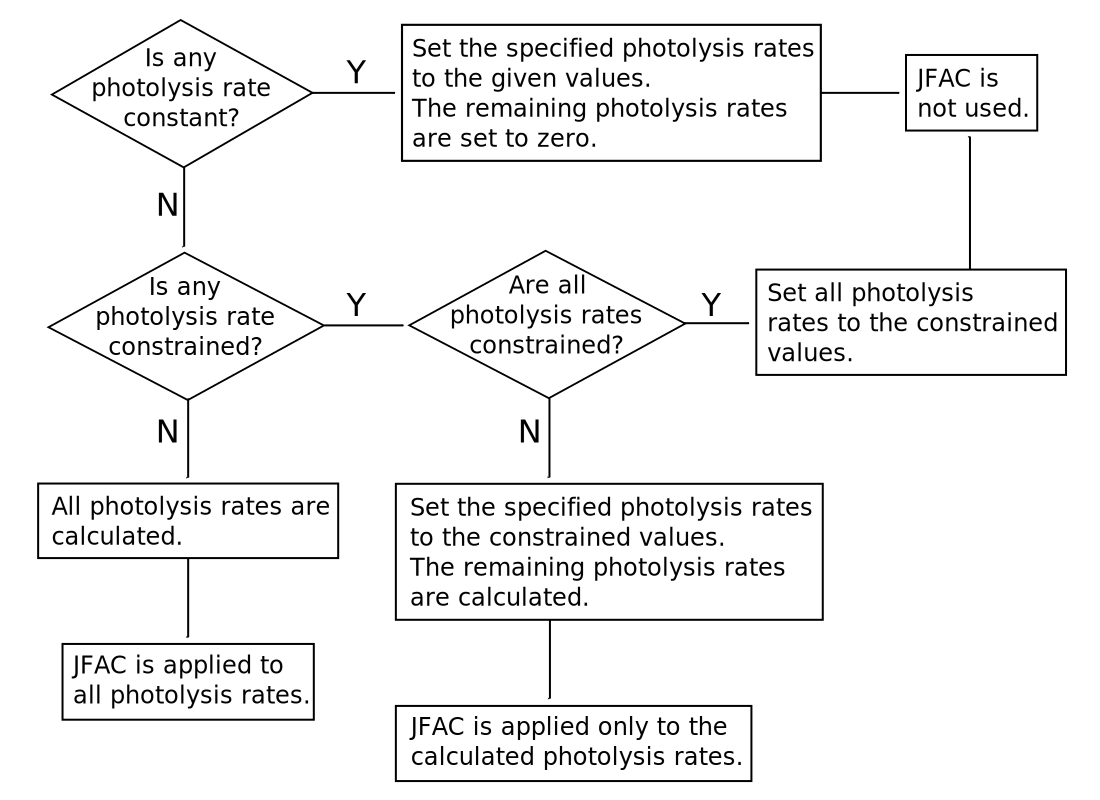
\includegraphics[width=0.85\textwidth]{photolysis-rates.png}
  \caption{Photolysis rates and \texttt{JFAC} in AtChem2.}
  \label{fig:photol}
\end{figure}

\subsection{Constant photolysis rates} \label{subsec:constant-photolysis-rates}

The typical scenario for constant photolysis rates is a lamp or solar
simulator in an environmental chamber. All the photolysis rates in the
chemical mechanism must be given a fixed value (in s$^{-1}$) in the
\texttt{photolysisConstant.config} file, otherwise they are
automatically set to zero (Fig.~\ref{fig:photol}). This approach
allows the user to model individual photolytic processes and/or to
account for lamps that emit only in certain spectral windows.

The format of \texttt{photolysisConstant.config} is described in
Sect.~\ref{subsec:photolysisconstant}. If the file is empty, the
photolysis rates are constrained or calculated by the model as
explained below.

\subsection{Constrained photolysis rates} \label{subsec:constrained-photolysis-rates}

All photolysis rates can be constrained to measured values. In this
case, the name of the constrained photolysis rate (e.g., \texttt{J2})
must be listed in the \texttt{photolysisConstrained.config} file
(Sect.~\ref{subsec:photolysisconstrained}); a corresponding file with the
constraint data must be present in the \texttt{model/constraints/photolysis/}

directory (see Sect.~\ref{subsec:constrained-variables} for details).

It is not always possible to measure -- and therefore to constrain --
all the required photolysis rates. The photolysis rates that are not
constrained (i.e. not listed in \texttt{photolysisConstrained.config})
are calculated by the model using the MCM parametrization, described
in the next section.

\subsection{Calculated photolysis rates} \label{subsec:calculated-photolysis-rates}

AtChem2 implements the parametrization of photolysis rates used by the
Master Chemical Mechanism, which is described in detail in the MCM
protocol papers \citep{jenkin_1997, saunders_2003}. Briefly, the
photolysis rate (\texttt{J}) is calculated as a function of the solar
zenith angle according to the following equation:

\begin{equation}
  J = l \times (cosX)^m \times e^{(-n \times secX)} \times \tau
\end{equation}

where $l$, $m$, $n$ are empirical parameters, $cosX$ is the cosine of
the solar zenith angle, $secX$ is the inverse of $cosX$ (i.e.
$secX\ =\ 1/cosX$) and $\tau$ is the transmission factor. The
transmission factor accounts for the loss of natural or artificial
light in some environmental chambers: the default value of $\tau$ is
1, which means there is perfect transmittance of light through the
chamber walls or windows. For more information, see the
\href{https://mcm.york.ac.uk/MCM/rates/photolysis}{photolysis page}
on the MCM website.

The empirical parameters are different for each version of the MCM: by
default, AtChem2 uses the empirical parameters of the MCM v3.3.1
(\texttt{mcm/photolysis-rates\_v3.3.1}), but it is possible to use the
empirical parameters of other MCM versions and to change the value of
$\tau$ -- see the file \texttt{mcm/INFO.md} for instructions.

The solar zenith angle (SZA) is the angle between the local vertical
(zenith) and the center of the sun. The SZA is measured in radians and
is calculated by the model from latitude, longitude, sun declination
and time of the day. These variables are set by the user in the
\texttt{model.parameters} file (Sect.~\ref{sec:model-parameters}). The
sun declination (\texttt{DEC}, Sect.~\ref{subsec:dec}) -- unless it is
constrained or set to a constant value -- is calculated by the
model. The calculations of the solar zenith angle and of the sun
declination are described in \citet{madronich_1993}.

\subsection{JFAC calculation} \label{subsec:jfac-calculation}

Measurements of ambient photolysis rates typically show short-term
variability due to changing meteorological conditions, such as clouds,
aerosol, etc\ldots \citep{sommariva_2020}. This information is
retained in the constrained photolysis rates, but it is not included
in the calculated ones. To take into account the ambient variability,
the calculated photolysis rates can be scaled by a constant or
time-dependent correction factor -- the environment variable
\texttt{JFAC} (Sect.~\ref{subsec:jfac}) -- defined as:

\begin{equation}
  \mathrm{JFAC} = \frac{j_{meas}}{j_{calc}}
\end{equation}

where $j_{meas}$ and $j_{calc}$ are the measured and calculated (with
the MCM parametrization, Sect.~\ref{subsec:calculated-photolysis-rates})
photolysis rates of a reference species. \cf{NO2} is often used as
reference because $j$(\cf{NO2}) is one of the most frequently measured
photolysis rates, in which case: \verb|JFAC = j(NO2)/J4|.

The parameter \texttt{JFAC} is by default set to 1, which means that
the calculated photolysis rates are not scaled; \texttt{JFAC} can be
set to any value between 0 and 1 (Sect.~\ref{subsec:jfac}), or it can
be constrained (Sect.~\ref{subsec:constrained-variables}). Note that
only the photolysis rates calculated with the MCM parametrization are
scaled by \texttt{JFAC}: the constrained and the constant photolysis
rates are never scaled (Fig.~\ref{fig:photol}).

AtChem2 can calculate \texttt{JFAC} automatically at runtime. To use
this option, edit the \texttt{environmentVariables.config} file
(Sect.~\ref{subsec:environmentvariables}) and set \texttt{JFAC} to the
name of the photolysis rate used as reference (e.g., \texttt{J4}).
The reference photolysis rate must also be constrained -- i.e. it must
be listed in the \texttt{photolysisConstrained.config} file
(Sect.~\ref{subsec:photolysisconstrained}) and the corresponding
constraint file must be present in the \texttt{model/constraints/photolysis/}
directory~\footnote{The calculation of \texttt{JFAC} at runtime does
  not work very well in the current version of AtChem2, especially in
  situations when the reference photolysis rate is highly variable and
  at sunrise/sunset. Therefore, it is recommended to calculate
  \texttt{JFAC} offline and then to constrain it (see issue
  \href{https://github.com/AtChem/AtChem2/issues/16}{\#16}).}.

% -------------------------------------------------------------------- %
\section{Config Files} \label{sec:config-files}

The configuration files contain the settings of the environment
variables, the chemical species, the photolysis rates, as well as the
model constraints and the model output. All the configuration files
have the extension \texttt{.config} and, by default, are located in
the \texttt{model/configuration/} directory. This directory also contains
the files with the settings of the model (\texttt{model.parameters})
and of the solver (\texttt{solver.parameters}), which are described in
Sect.~\ref{sec:model-parameters} and Sect.~\ref{sec:solver-parameters},
respectively.

Usually, the \texttt{model/configuration/} directory is also the same
as the \sharedir, which contains the pre-compiled chemical mechanism
generated during the \hyperref[subsec:build-process]{build process}.
The names and paths of these directories can be modified by the user,
as explained in Sect.~\ref{subsec:model-directory}. The content and
the format of each \texttt{.config} file are described below.

\subsection{environmentVariables.config} \label{subsec:environmentvariables}

This file specifies the settings of the environment variables, i.e.
the physical parameters of the model. The file has three columns: the
first two are the ID number and the name of the environment variable.
The third column -- the only one that should be modified by the
user -- contains the corresponding value. The possible values of each
environment variable are detailed in Sect.~\ref{sec:environment-variables}.
For example:

\begin{verbatim}
1   TEMP         293
2   PRESS        1013
3   RH           CONSTRAINED
4   H2O          CALC
5   DEC          CALC
6   BLHEIGHT     8e+4
7   DILUTE       NOTUSED
8   JFAC         CONSTRAINED
9   ROOF         OPEN
10  ASA          2e-5
\end{verbatim}

If an environment variable is constrained, there must be a
corresponding data file in the \texttt{model/constraints/environment/}
directory, except for \texttt{JFAC} whose data file should go in the
\texttt{model/constraints/photolysis/} directory. For more
information, go to Sect.~\ref{subsec:constrained-variables}.

\subsection{initialConcentrations.config} \label{subsec:initialconcentrations}

This file specifies the initial concentrations (in molecule cm$^{-3}$)
of the chemical species. The file has two columns: the first column is the
name of the initialized species, the second column is the corresponding
concentration at the \textbf{model start time}, which is defined
in the \texttt{model.parameters} file (Sect.~\ref{sec:model-parameters}).
For example:

\begin{verbatim}
O3      1.213e+12
NO      378473308.14
NO2     86893908168.9
CH4     4.938e+13
\end{verbatim}

Not all chemical species need to be initialized: those that are not
listed in \texttt{initialConcentrations.config} are assumed to have an
initial concentration of zero molecule cm$^{-3}$. It is also not
necessary to initialize the chemical species that are set to constant
values or constrained to measured concentrations, i.e. those listed in
\texttt{speciesConstant.config} and/or \texttt{speciesConstrained.config}
(see below).

\subsection{outputRates.config} \label{subsec:outputrates}

This file lists the chemical species for which detailed
production/loss rates are required~\footnote{In version 1.0 and
  earlier, these species were listed in two separate files:
  \texttt{productionRatesOutput.config}, \texttt{lossRatesOutput.config}.}.
The file has one column, with one species per line. For example:

\begin{verbatim}
OH
HO2
NO3
\end{verbatim}

The frequency of this output is controlled by \textbf{rates output step size}
in the \texttt{model.parameters} file (Sect.~\ref{sec:model-parameters}).
The corresponding output files -- called \texttt{productionRates.output}
and \texttt{lossRates.output} -- are formatted to facilitate the rate
of production and destruction analysis of selected species. For more
information, go to Sect.~\ref{subsec:ropa-roda}.

\subsection{outputSpecies.config} \label{subsec:outputspecies}

This file~\footnote{Called \texttt{concentrationOutput.config} in
  version 1.0 and earlier.} lists the chemical species for which the
calculated concentration (in molecule cm$^{-3}$) is required. The file
has one column, with one species per line. For example:

\begin{verbatim}
O3
NO2
CH4
OH
HO2
\end{verbatim}

The frequency of this output is controlled by the \textbf{step size} parameter
in the \texttt{model.parameters} file (Sect.~\ref{sec:model-parameters}).
Constrained chemical species may be listed in \texttt{outputSpecies.config},
which can be useful for diagnostic and debugging purposes. Note that
the photolysis rates, the environment variables, \cf{H2O}, and the
\cf{RO2} sum are always output by the model (Sect.~\ref{sec:output}).
Therefore, there is not a \texttt{.config} file to set the output of
these variables and they \emph{should not} be listed in
\texttt{outputSpecies.config}.

\subsection{photolysisConstant.config} \label{subsec:photolysisconstant}

This file lists the photolysis rates that are set to constant values
(Sect.~\ref{subsec:constant-photolysis-rates}). The file has three
columns: the first column is the ID number of the photolysis rate, the
second column is the value of the photolysis rate (in s$^{-1}$), the
third column is the name of the photolysis rate. The ID numbers and
the names of the photolysis rates follow the
\href{https://mcm.york.ac.uk/MCM/rates/photolysis}{MCM designation}.
For example:

\begin{verbatim}
1     2.5e-5     J1
4     8.7e-3     J4
7     1.8e-3     J7
\end{verbatim}

The photolysis rates that are not listed in \texttt{photolysisConstants.config}
are automatically set to zero (Fig.~\ref{fig:photol}). If no photolysis rate
is set to constant, the file should be empty.

\subsection{photolysisConstrained.config} \label{subsec:photolysisconstrained}

This file~\footnote{Called \texttt{constrainedPhotoRates.config} in
  version 1.0 and earlier.} lists the photolysis rates that are constrained
(Sect.~\ref{subsec:constrained-photolysis-rates}). The file has one column,
with one photolysis rate per line. The names of the photolysis rates follow
the \href{https://mcm.york.ac.uk/MCM/rates/photolysis}{MCM designation}.
For example:

\begin{verbatim}
J1
J4
J7
\end{verbatim}

If a photolysis rate is constrained, there must be a corresponding
constraint file in the \texttt{model/constraints/photolysis/}
directory (Sect.~\ref{subsec:constrained-variables}). The photolysis
rates that are not listed in \texttt{photolysisConstrained.config} are
calculated using the MCM parametrization (Fig.~\ref{fig:photol}). If
no photolysis rate is constrained, the file should be empty.

\subsection{speciesConstant.config} \label{subsec:speciesconstant}

This file~\footnote{Called \texttt{constrainedFixedSpecies.config} in
  version 1.0 and earlier.} lists the chemical species that are set to
constant concentrations. The file has two columns: the first column is
the list of constant species, the second column is the corresponding
concentration (in molecule cm$^{-3}$). For example:

\begin{verbatim}
CH4     4.4e+13
CO      2.5e+12
H2      1.2e+13
\end{verbatim}

The chemical species that are set to a constant value do not need to
be initialized: the values set in \texttt{speciesConstant.config}
override those set in \texttt{initialConcentrations.config}. If no
chemical species is set to constant, the file should be empty.

\subsection{speciesConstrained.config} \label{subsec:speciesconstrained}

This file~\footnote{Called \texttt{constrainedSpecies.config} in
  version 1.0 and earlier.} lists the chemical species that are
constrained. The file has one column, with one species per line. If a
chemical species is constrained, there must be a corresponding
constraint file in the \texttt{model/constraints/species/} directory
(Sect.~\ref{subsec:constrained-variables}). For example:

\begin{verbatim}
CH4
CO
H2
\end{verbatim}

The chemical species that are constrained do not need to be
initialized: the values set in \texttt{speciesConstrained.config}
override those set in \texttt{initialConcentrations.config}. If no
chemical species is constrained, the file should be empty.
